\subsection{Electromagnetic Calorimeter}
%\writer{Jean Claude Brient, Wataru Ootani}{3}

\subsubsection{Silicon option (SiECAL)}

In the past 5 years the Silicon option of the electromagnetic calorimeter has focused on the design and construction of technological prototypes of the detector including beam tests. The current technological developments have led to choosing 20cm wafers for making the diode matrices, with a standard thickness of up to 725 micrometers. When applied to ILD this would result in a slightly thicker EM calorimeter than foreseen in the baseline design, and is one of the motivations to reduce the numbers of layers from 30 to 26 (see section 5.1.2).

A fully integrated layout of the detection board has been designed with the required dimension of 16 x 16 $cm^2$ corresponding to 1024 channels (Figure~\ref{fig:det:SiWECAL_proto} top). The board hosts 16 SKIROC ASICs developed by OMEGA~\cite{Callier:2011zz,Suehara:2018mqk} to process 64 channels each. A calorimeter prototype based on 10 such detection layers has been built~\cite{Boudry:2014bxa,Poeschl:2015jma} (Figure~\ref{fig:det:SiWECAL_proto} bottom) and beam-tested on several occasions at DESY and CERN, including a combined test with a SDHCAL prototype of the hadronic calorimeter (next section).   
\begin{figure}[t!]
\centering
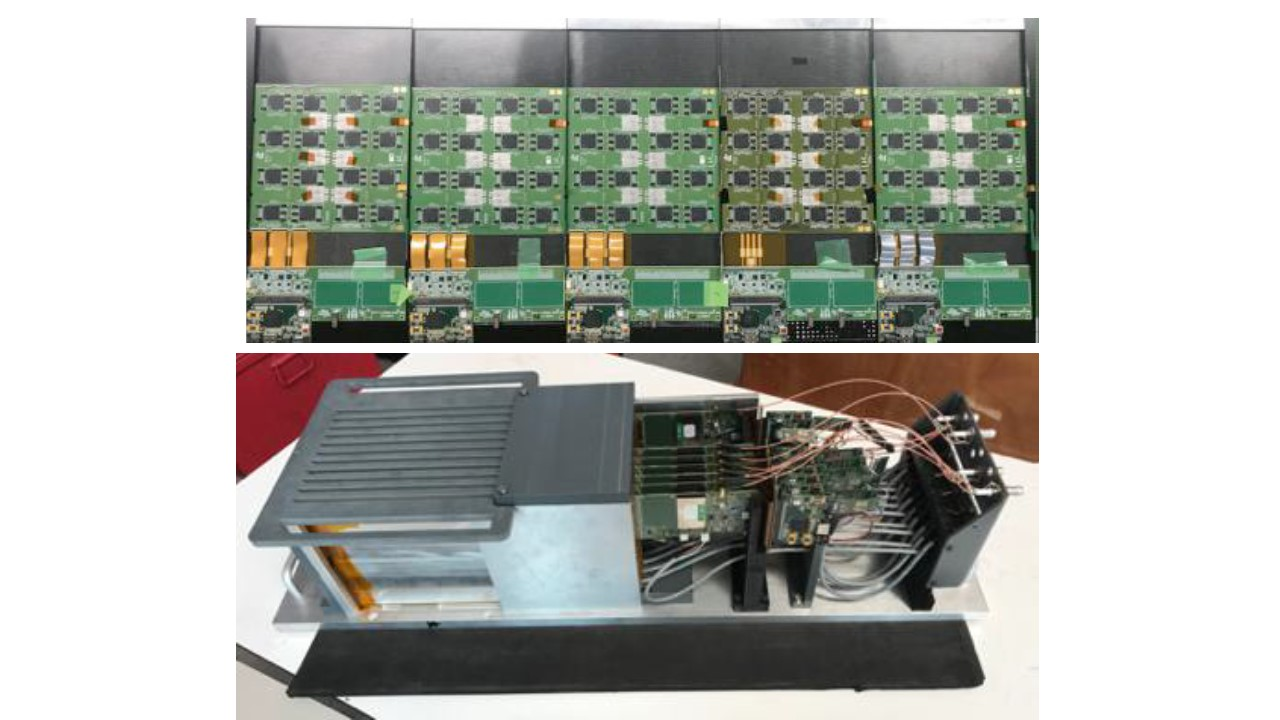
\includegraphics[width=1.0\hsize]{Detector/fig/SiWECAL_proto.jpg}
\caption{Technological prototype of the SiECAL. Top: set of integrated sensor\&readout boards; bottom: 10-layers calorimeter prototype used in beam tests at DESY and CERN.}
\label{fig:det:SiWECAL_proto}
\end{figure}

The response of this technological prototype to particles behaves as expected~\cite{Kawagoe:2019dzh}. A signal-to-noise ratio of 20 is measured for MIPs in single pads (Figure~\ref{fig:det:SiWECAL_signals} left). Such a large signal/noise ratio of MIPs is important for isolated particle identification in particle flow energy reconstruction. First response to high energy electrons has recently been measured at CERN in a combined test with the SDHCAL (Figure~\ref{fig:det:SiWECAL_signals} right). The beam tests have also been used to validate the power pulsing of the front-end electronics required to minimize heat production within the calorimeter. A new version of the detector slabs is currently in production from a joint development in LLR and Kyushu. A total number of 20 detection layers could be reached in the coming year. This will allow the construction of a full ECAL prototype to be used in test beams for measurements of the energy resolution.

\begin{figure}[t!]
\centering
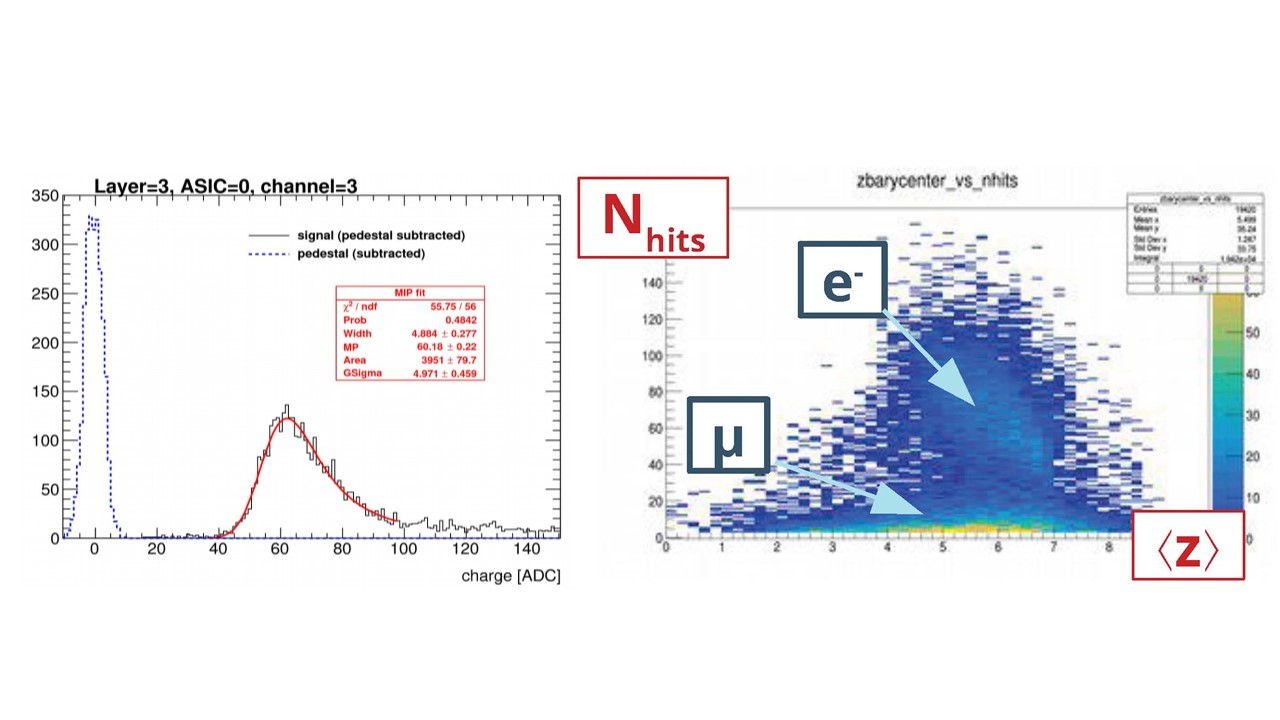
\includegraphics[width=1.0\hsize]{Detector/fig/SiWECAL_signals.jpg}
\caption{Particle response of the SiECAL prototype: MIP response of a single pad (left) and shower profile of muons and 80 GeV electrons (right).}
\label{fig:det:SiWECAL_signals}
\end{figure}

More developments are ongoing to reach the requirements of the full-size ILD detector. The layout of the sensitive layer diode matrices has been revisited since the technological prototype construction. A large detector slab with dimensions similar to those of the calorimeter modules has been built and tested with MIPs~\cite{Balagura:2017vvf} (Figure~\ref{fig:det:SiWECAL_dev} right). A 10\% signal drop has been observed along the full length of the slab and could be attributed to power voltage drops and clock reflections. An updaded long slab is under construction to correct these effects and validate the solutions. In addition, an electronics readout concentrator and interface board with the detector slabs, located at the end of the slabs, is under development in LAL with a size and performance close to those needed for the ILD detector. Ultra thin detection boards with ASICs integrated within the PCB have also been developed and are under test with cosmics (Figure~\ref{fig:det:SiWECAL_dev} left). Provided industrial aspects are under control, they may allow even more compact layouts of the electromagnetic calorimeter. 

\begin{figure}[t!]
\centering
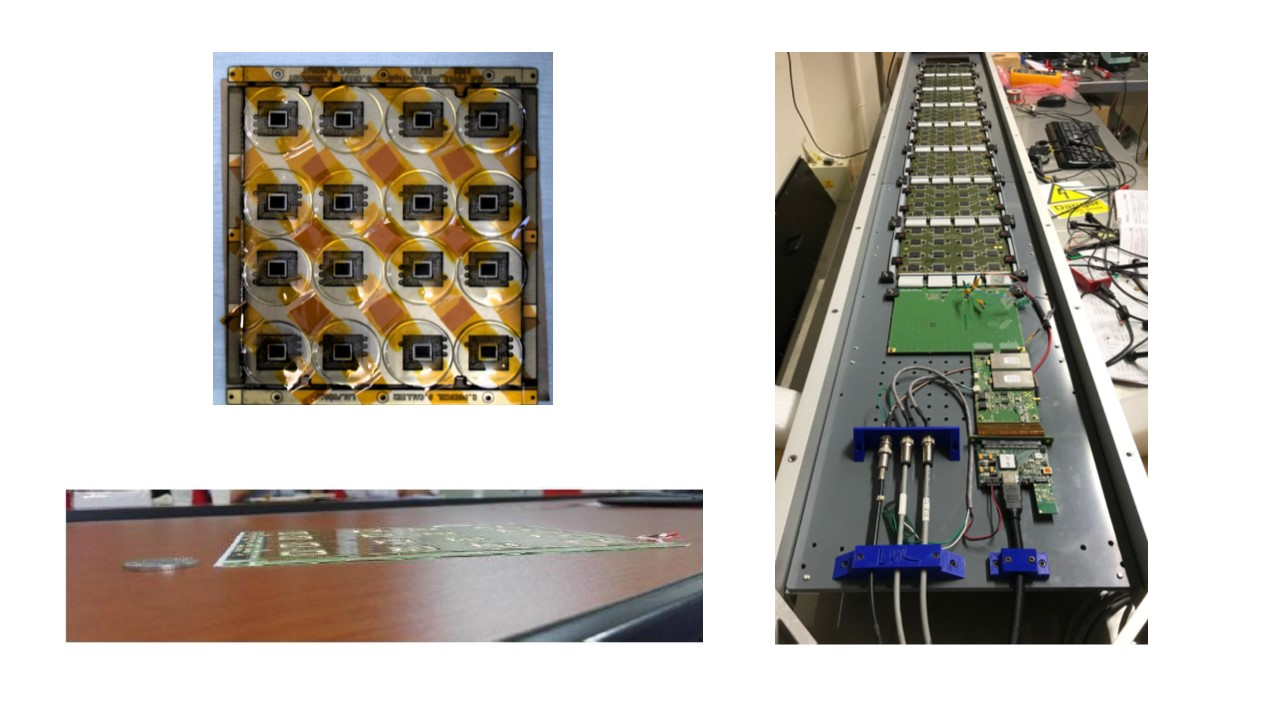
\includegraphics[width=1.0\hsize]{Detector/fig/SiWECAL_dev.jpg}
\caption{SiECAL developments towards the final detector: thin chip-on-board sensors (left) and long slabs corresponding to ILD dimensions (right).}
\label{fig:det:SiWECAL_dev}
\end{figure}

The Silicon technology developed for ILD has been retained as the baseline for the electromagnetic section of the CMS High Granularity Calorimeter (HGCAL) upgrade~\cite{Collaboration:2293646}. The HGCAL layout is based on hexagonal readout modules with a technology similar to the ILD one. It incorporates a new version of the SKIROC ASIC with a sub-ns timing functionality which may also be of interest for the ILD detector. A HGCAL prototype of 27 layers has been successfully tested by CMS in a combined beam test at CERN with the AHCAL ILD prototype (next section). The full HGCAL represents a 10\% prototype of the ILD SiECAL as regards the number of channels. Its construction will be a strong asset to validate the large scale assembly and fabrication processes for ILD. 

%\textit{Sc-ECAL results from new detector unit in construction.}

\subsubsection{Scintillator option (ScECAL)}

Similarly to the silicon option, the scintillator option of the electromagnetic calorimeter,
after the validation of the concept using the physics prototype,
has focused its R\&D towards a technological prototype 
with fully integrated detection layers. 
The design of the detection layer is based on an integrated readout board, 
called ECAL base unit (EBU), of $18\times18\,\mathrm{cm}^2$ 
with four SPIROC ASICs developed by OMEGA group\cite{ild:bib:spiroc} on which 144 scintillator strips 
($5\times45\times2\,\mathrm{mm^3}$ each) coupled to SiPMs are mounted.

Notable progresses have recently been made on the SiPMs for the ScECAL. 
MPPCs with a smaller pixel pitch of 10 or $15\,\mu\mathrm{m}$ have been developed 
by Hamamatsu Photonics K.K, which can provide a larger dynamic range required 
for the ScECAL\cite{ild:bib:hdmppc}. 
Further improvements have been made for the most recent small-pixel MPPCs, 
including reduced optical cross-talk by a trench structure between pixels, 
lower dark noise and higher PDE, which have been confirmed by the prototype tests.

In the previous prototype studies, the SiPM was attached to the side edge 
of the strip. 
New designs of the SiPM readout at the bottom side of the strip 
are being developed for more uniform response and a better compatibility 
with future large-scale production.
Especially a recently proposed design based on a strip 
with a dimple directly coupled to a surface-mounted SiPM on the PCB, 
which is similar to the SiPM-on-tile technology of AHCAL,
shows a promising performance.

Low cost and high light yield plastic scintillator materials are also being developed 
for the ScECAL.
The development focuses on the polystyrene-based scintillator 
produced by the injection moulding method, which is suitable 
for large-scale production. 
A reasonably high light yield of 65--70\% compared to that of 
the commercial PVT-based scintillator has been achieved 
by optimizing the production parameters. 

Detection layer prototypes have been developed 
with the small pixel MPPCs ($15\,\mu\mathrm{m}$ pixel pitch) 
as shown in the left of Figure~\ref{fig:det:ScWECAL_prototype}.
A prototype layer was tested in positron beams of 50--800\,MeV 
at ELPH of the Tohoku University.
The right of Figure~\ref{fig:det:ScWECAL_prototype} shows the typical charge distribution 
obtained for the positron beam where the MIP peak is well separated 
from the pedestal.

\begin{figure}[htb]
\centering
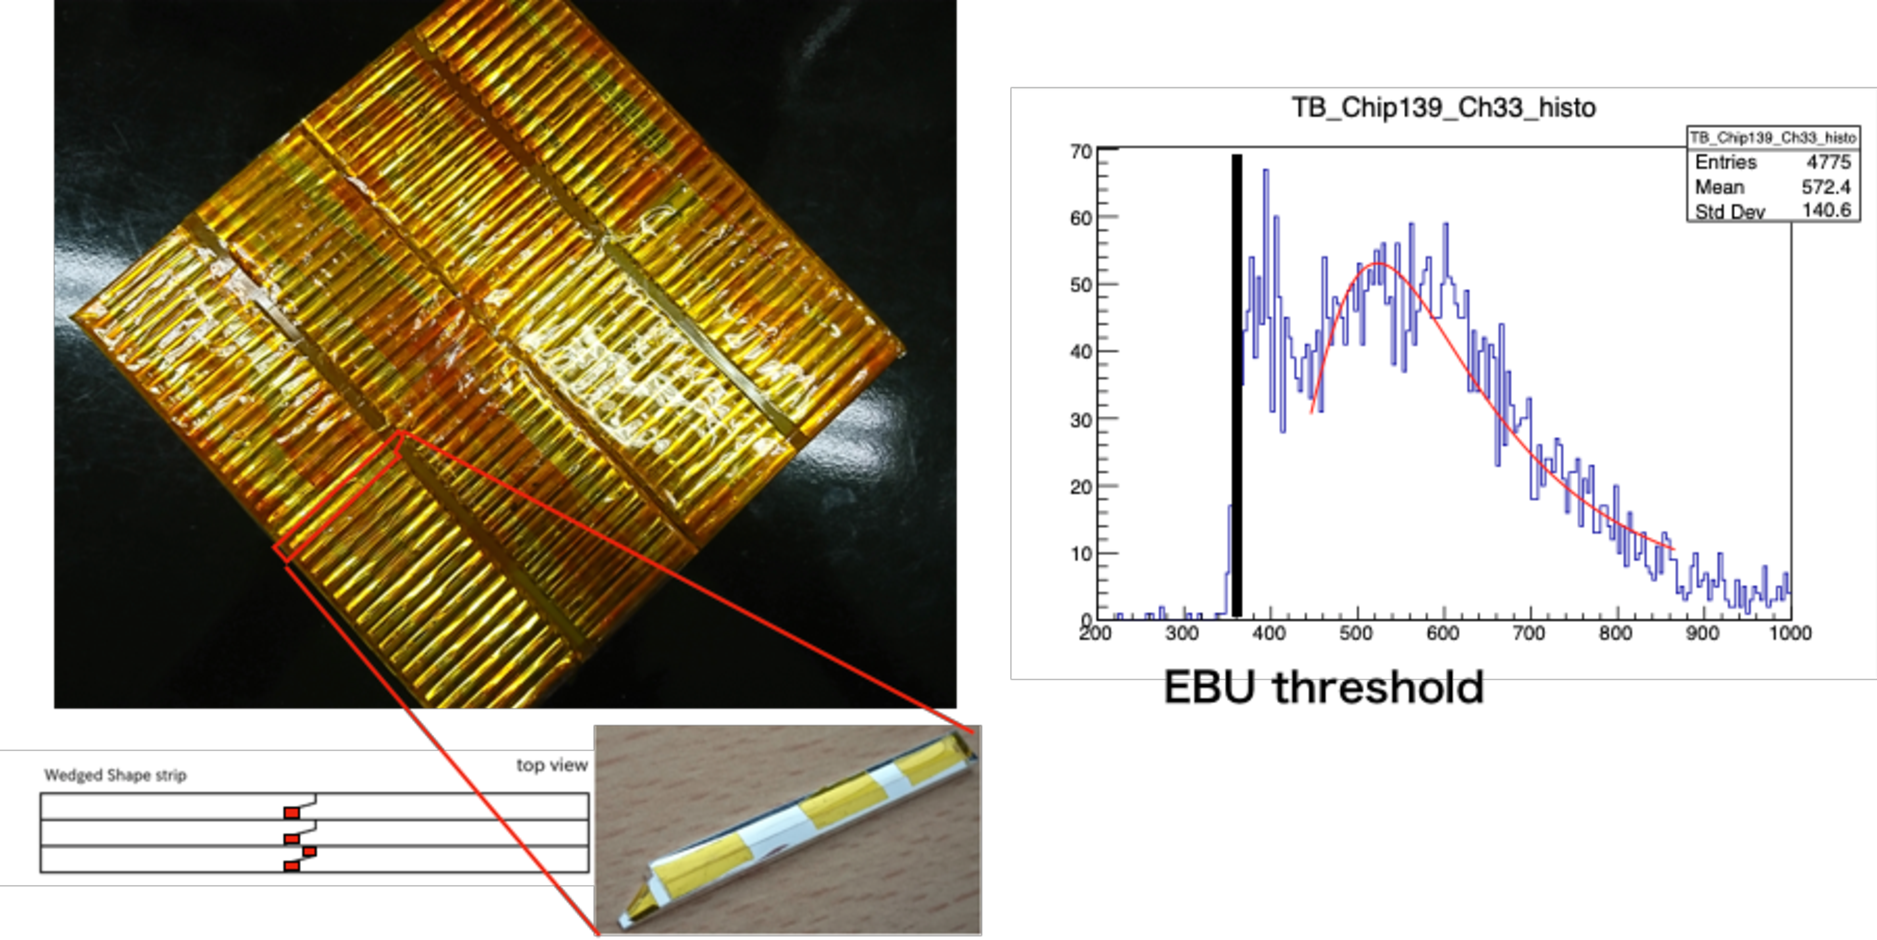
\includegraphics[width=1.0\hsize]{Detector/fig/ScWECAL_prototype.pdf}
\caption{(Left) Prototype detection layer with small pixel MPPCs  
   and (right) typical charge distribution obtained for positron beam 
where a MIP peak is well separated from the pedestal.}
\label{fig:det:ScWECAL_prototype}
\end{figure}


A fully integrated technological prototype with 30 alternating absorber and detection 
layers is planned to be constructed 
as a joint effort with the ScECAL R\&D for CEPC 
to demonstrate the performance of the ScECAL technology 
and its scalability to the full-size detector. 

\vspace{2cm}
